\documentclass{article}

\usepackage[margin=1in]{geometry}
\usepackage{enumitem}

\usepackage{amsmath}
\usepackage{amsfonts}
\usepackage{amssymb}
\usepackage{graphicx}
\usepackage{caption}
\usepackage{subcaption}

\newcommand{\tr}{^\mathsf{T}}
\DeclareMathOperator{\var}{V@R}
\DeclareMathOperator{\avar}{AV@R}
\newcommand{\Ex}{\mathbb{E}}
\newcommand{\one}{\mathbf{1}}
\newcommand{\zero}{\mathbf{0}}
\newcommand{\eye}{\mathbf{I}}
\newcommand{\states}{\mathcal{S}}
\newcommand{\actions}{\mathcal{A}}
\newcommand{\Real}{\mathbb{R}}
\newcommand{\opt}{^{\star}}

\setlength{\parskip}{2mm plus1mm minus1mm}
\setlength{\parindent}{0cm} 

\title{Optimization for CVaR IRL}
\author{}

\begin{document}
	\maketitle
	
	
\section{Notation}	
	We use the following notation:
	\begin{itemize}
		\item States $\states = \{1, \ldots, S \}$
		\item Actions $\actions = \{ 1, \ldots, A\}$
		\item $\Delta^k$ probability simplex in k-dimensions.
		\item Initial distribution: $p_0 \in \Delta^S$
		\item Rewards: $r: \states\times\actions \to \Real$
		\item Policy: $\pi: \states \times \actions \to [0,1]$  \textbf{[Double check other notation to make it work for stochastic policies]}
		\item Rewards for policy $\pi$: $r_\pi(s) = \mathbb{E}_{a \sim \pi(s)} r(s, a)$
		\item Expert's policy $\pi_{E}: \states \to \actions$
		\item Transition probability for a policy $\pi$: $P_\pi$, treated as a matrix, defined as:
		\[ P_\pi(s,s') = \mathbb{E}_{a \sim \pi(s)} P(s,a,s') = \sum_a \pi(a|s) P(s,a,s'	)\]
		\item Occupancy frequency for a policy: $u_\pi = (I - \gamma P_\pi \tr)^{-1} p_0$. This can be derived by noting that the Markov Chain stationary distribution over states $u_\pi$ satisfies the following equation at equilibrium: $u_\pi = p_0 + \gamma P^T_\pi u_\pi$. Solving for $u_\pi$ yields the above equation. 
		\item If we want the state-action occupancies we can solve for these similarly as $u_\pi = p_0 + \gamma P^T_\pi u_\pi$ and $u(s,a) = u_\pi \cdot \pi(a|s)$.
		\item Linear feature matrix with rows as states and columns as features: $\Phi \in \Real^{S\cdot A \times k}$, where $k$ is the number of features
		\item Assume that the rewards are approximated as $r = \Phi w$ for some $w\in\Real^k$
		\item Feature counts: $\mu_\pi = \Phi\tr u_\pi$. Here $\mu_\pi \in \Real^k$
		\item Value function $v_\pi = (I - \gamma P_\pi)^{-1} r_\pi $. This can be derived via the bellman equation for values: $v_\pi = r_\pi + \gamma P_\pi v_\pi$ and solving for $v_\pi$.
		\item Return for a specific policy and rewards: $\rho(\pi, r) = p_0\tr v = u_\pi\tr r_\pi$
	\end{itemize}
	
	
	Now, assume that $R$ is the random variable representing the reward. The posterior can be derived using Bayesian IRL. Let $R_1, R_2, R_3, \ldots$ be samples from the posterior distribution.


\section{Value at Risk}
When dealing with risk we will assume that lower values are worse (riskier), thus we will want to maximize the Value at Risk or Conditional Value at Risk since tails to the left are  bad. We will define $\alpha$-Value at risk as the $(1-\alpha)$ quantile worst-case outcome. Thus, the $\alpha$-VaR is such that 
\begin{equation}
\alpha\text{-VaR}[X] = \sup \{x : Pr(X \geq x) \geq \alpha\}
\end{equation}
	
	Given policy $\pi$, our AAAI'19 paper \cite{Brown2017} focused on finding a high-confidence lower bound on:
	\[ \var\left[\rho(\pi, R) - \rho(\pi^*_R, R) \right] ,\]

This is not quite the same as finding a lower bound on 
	\[ \var\left[\rho(\pi, R) - \rho(\pi_E, R) \right] ,\]	

	where $R$ is the random variable distributed according to the posterior from the Bayesian IRL. This second form is interesting because we may be able to do better than the expert. We don't want to match the risk of the expert, rather we want to minimize our risk with the expert as the baseline. \textbf{Can we do the same thing as our AAAI paper by reusing the BIRL $\pi^*$ for each policy? I think so. We just adjust the objective so instead of $u_E$ we use $u_{\pi^*}$, right?} We will denote the posterior distribution $p$; and generally assume that $p$ is a probability distribution over a finite number of samples from the posterior distribution, e.g. a uniform distribution over $n$ samples from MCMC. In \cite{Brown2017} we derive finite-sample bounds in terms of the number of samples from the posterior distribution. Unfortunately, $\var$ is not convex and thus is hard to optimize.


\section{Average Value at Risk}
Average Value at Risk ($\avar$) is a convex coherent risk measure. It is also commonly referred to as Conditional Value at Risk, expected tail risk, or expected shortfall. It is convex, and is a lower bound on $\var$. It can be also preferable because it does not ignore how heavy the tail of the distribution is. $\var$ only considers the quantile, but ignores any outcome that may be worse than that.
	
	The intuitive (but not entirely correct) definition of $\avar$ (the same as CVaR) is:
	\[ \avar_\alpha[X] = \Ex\left[ X ~\mid~ X \le \var_\alpha[X]\right] ~.\]
	This only works for atomless distributions such that no $\omega$ has a positive probability (i.e. most continuous distributions). However, we are interested in maximizing $\avar$ given a finite number of samples from the posterior distribution $P(R|D)$. The correct convex definition of $\avar$ that works for any distribution (discrete or continuous) is:
	\[ \max_{\sigma}\; \left( \sigma - \frac{1}{1-\alpha} p\tr [\sigma \cdot \one - x ]_+ \right) ~,\]
	where $[\cdot]_+$ is an element-wise non-negative part of the vector $x$: $[x]_+ = \max \{x, \zero\}$. 
	
	
	
	A popular way to analyze and use coherent risk measures is to look at their robust representation:
	\[ \avar_\alpha[X] = \min_{q\in\mathcal{Q}} \Ex_q[X]~, \]
	which is the expectation with respect to a worst-case distortion of the nominal probability distribution $p$. For $\avar$ the set $\mathcal{Q}$ is defined as:
	\[ \mathcal{Q} = \left\{ q \in \Delta^n ~\mid~ q \le \frac{1}{1-\alpha} p \right\} ~, \]
	where $\Delta^n$ is the probability simplex over $\mathbb{R}^n$ and $p \in \Delta^n$. You can think about this as follows: when alpha is 0 then $q\leq p$ and since $\sum q = \sum p = 1$ and $q \geq 0$, we must have $q = p$. Thus CVaR is just $\min_{q=p}\mathbb{E}_q[X] = \mathbb{E}_p[X]$. Just the nominal expectation since VaR with alpha = 0 is the biggest possible value of X so CVaR is just the expectation of X. As you make alpha larger it gives q more wiggle room. As alpha goes to 1 you make 1/(1-alpha) go to infinity so q can choose to put all the probability mass on very unlikely outcomes. Because it is trying to minimize expectation under this warped distribution it will put as much weight as it can on these worst outcomes and can focus more on unlikely outcomes as alpha goes to 1. 
	
	Lets say that the goal is to find the best policy and we want to minimize $\avar$ of the ``robust baseline regret''~\cite{Ho2016,Petrik2016,Syed2008}. We called this a robust baseline regret but this is just the standard objective in IRL:
	\begin{equation} \label{eq:holy_grail}
	\max_{\pi} \avar_\alpha\left[ \rho(\pi, R) - \rho(\pi_E, R) \right] 
	\end{equation}
	
	
	We can formulate \eqref{eq:holy_grail} as a linear program following the next steps. Recall the one to one correspondence between randomized policies $\pi: \mathcal{S} \to \Delta^A$ (where $A$ is the number of actions) and the occupancy frequencies $u$~\cite{Puterman2005}. That means that $\max_{\pi} \rho(\pi, r)$ corresponds to the following linear program~\cite{Puterman2005}:
	\[\max_{u:\states\times\actions\to\Real} \left\{ r\tr u ~\mid~ \sum_{a\in\mathcal{A}} (\eye - \gamma\cdot P_a\tr) u_a = p_0, u \ge \zero \right\}~. \]
	
I'm currently solving this via SciPy's built in LP solver as follows:

\begin{eqnarray}
\min_{u:\states\times\actions\to\Real}&& -r\tr u \\
\text{s.t.}&&\begin{bmatrix}
(I - \gamma P_{a_1}\tr), \ldots, (I - \gamma P_{a_m}\tr)
\end{bmatrix}
\begin{bmatrix}
u_{a_1} \\
\vdots\\
u_{a_n}
\end{bmatrix}
= p_0 \\
&& u \geq \zero
\end{eqnarray}
where $u_{a} = [u_{(s_1, a)}, u_{(s_2, a)}, \ldots u_{(s_n, a)}]\tr$. 

	Using the same approach as the linear program above, we can formulate \eqref{eq:holy_grail} as a linear program following these steps. Let $R$ be a matrix $(S\cdot A) \times n$ of all sampled posterior rewards $R$. That is, each column of $R$ represents one sample of the vector over rewards for each state and action pair. \eqref{eq:holy_grail} becomes:
	\begin{equation} \label{eq:lp_objective}
	\max_{u,\sigma} \left\{ \sigma -\frac{1}{1-\alpha} p\tr \left[\sigma\cdot\one - R\tr u  + R\tr u_E \right]_+  ~\mid~ \sum_{a\in\mathcal{A}} (\eye - \gamma\cdot P_a\tr) u_a = p_0, u \ge \zero \right\}~.  
	\end{equation}
	This is a linear program which works in the tabular case. This can be written more explicitly as 
	
\begin{eqnarray}
\max_{\sigma, u}&& \sigma - \frac{1}{1-\alpha}p\tr z \\
\text{s.t.}&& z \geq \sigma \one - R\tr(u - u_E)\\
&&\begin{bmatrix}
(I - \gamma P_{a_1}\tr), \ldots, (I - \gamma P_{a_m}\tr)
\end{bmatrix}
\begin{bmatrix}
u_{a_1} \\
\vdots\\
u_{a_n}
\end{bmatrix}
= p_0 \\
&& u \geq \zero \\
&& z \geq \zero 
\end{eqnarray}		
	
	
I'm using SciPy to solve this LP in the following form:

\begin{eqnarray}
\min_{\sigma, u}&& -\sigma + \frac{1}{1-\alpha}p\tr z \\
\text{s.t.}&& - R\tr u + \sigma \one  - z  \leq -R\tr u_E\\
&&\begin{bmatrix}
(I - \gamma P_{a_1}\tr), \ldots, (I - \gamma P_{a_m}\tr)
\end{bmatrix}
\begin{bmatrix}
u_{a_1} \\
\vdots\\
u_{a_n}
\end{bmatrix}
= p_0 \\
&& u \geq \zero \\
&& z \geq \zero 
\end{eqnarray}	
	
	
	The optimal risk-averse IRL policy $\pi\opt$ can be constructed from an optimal $u\opt$ solution to \eqref{eq:lp_objective} as:
	\begin{equation} \label{eq:policy_from_u}
	\pi\opt(s,a) = \frac{u\opt(s,a)}{\sum_{a'\in\mathcal{A}} u\opt(s,a') }~. 
	\end{equation}
	

\subsection{Linear Reward Function Approximation}
	
	The linear program can be easily extended to linear approximation by assuming that $r = \Phi w$ is which case the return becomes $u\tr r = u\tr \Phi w = \mu\tr w$.
	
	
	Using the same approach as the linear program above, we can formulate \eqref{eq:holy_grail} as the following linear program,	
	
	\begin{equation} \label{eq:lp_objective}
	\max_{u,\sigma} \left\{ \sigma -\frac{1}{1-\alpha} p\tr \left[\sigma\cdot\one - R\tr u  + R\tr u_E \right]_+  ~\mid~ \sum_{a\in\mathcal{A}} (\eye - \gamma\cdot P_a\tr) u_a = p_0, u \ge \zero \right\}~.  
	\end{equation}
	
where 
\begin{equation}
R =
\begin{bmatrix}
\Phi w_1, \cdots, \Phi w_n 
\end{bmatrix}
\end{equation}

\textbf{Can we reformulate it in terms of expected feature counts instead of state-action occupancies? Is there any benefit to this?}

\subsection{Non-linear reward function approximation}
	
	This formulation can be extended to non-linear approximation using a similar approach as GAIL, I think. The key is the dual representation of $\avar$ naturally maps to an adversarial algorithm. 

\subsection{Recovering Rewards}

The question is how to recover the reward vector the would generate the AVaR return. One possibility is to use the dual representation of AVaR. Let $\pi\opt$ be the optimal solution to \eqref{eq:lp_objective} as in \eqref{eq:policy_from_u}. Let:
\[ \mathcal{Q} = \left\{ q \in \Delta^n ~\mid~ q \le \frac{1}{1-\alpha} p \right\} ~. \]
Then to get the reward, let $\pi\opt$ be the optimal solution to \eqref{eq:lp_objective}. Then one needs to solve:
\begin{equation} \label{eq:q_value}
\avar_\alpha\left[ \rho(\pi\opt, R) - \rho(\pi_E, R) \right] = \min_{q\in\mathcal{Q}} \Ex_{R \sim q} \left[ \rho(\pi\opt, R) - \rho(\pi_E, R) \right]~.
\end{equation}
\textbf{It seems like this should be minimize, right? I'm changing it for now.}
Another way to write the expectation would be as follows:
\[ \Ex_{R \sim q} \left[ \rho(\pi\opt, R) - \rho(\pi_E, R) \right] = \sum_{i=1}^n q_i \left( \rho(\pi\opt, r_i) - \rho(\pi_E, r_i) \right)~, \]
where $r_i$ is the $i$-th posterior sample.


Let $q\opt$ be the optimal solution to the linear program in \eqref{eq:q_value}. Using the fact that $\rho$ is linear in $r$, we get:
\[ \Ex_{R \sim q\opt} \left[ \rho(\pi\opt, R) - \rho(\pi_E, R) \right] =  \rho\left(\pi\opt, \Ex_{R \sim q\opt}[R]\right) - \rho\left(\pi_E, \Ex_{R \sim q\opt}[R]\right)~.\]
That means that $\Ex_{R \sim q\opt}[R] = \sum_i q_i R_i$ is the worst-case reward.

So does this mean that $\pi^*_{cvar}$ is optimal wrt $\Ex_{R \sim q\opt}[R]$ or that it is optimal wrt maximizing the CVaR robust baseline regret wrt this reward? It must be the latter, right? Actually, since $R_{cvar}\tr u_E$ is constant shouldn't maximizing one be equivalant to maximizing the other? Why doesn't it work out in code? The learned policy doesn't match what you would get by just maximizing policy for $R_{cvar}$. 

One possible issue that I've noticed is that there might be multiple optimal solutions for $R_{cvar}$. This is because if there are two different reward functions that lead to the same policy loss then $q^*$ can blend them any way. However, this seems to be able to lead to different optimal policies. It would be nice to have a reward function that when optimized would recover the solution to the CVaR policy, but maybe that is not possible?

\subsection{Dual}

So, after talking with Marek it turns out that to get the reward that, when optimized, results in the CVaR optimal policy, we need to solve the dual problem:

\begin{eqnarray}
\min_{v, q}&& p_0^T v - u_E^T R q\\
\text{s.t.}&& \sum_{i=1}^n q = 1 \\
&& q \leq \frac{1}{1-\alpha}p\\
&&\begin{bmatrix}
(I - \gamma P_{a_1})\\
\vdots \\
(I - \gamma P_{a_m})
\end{bmatrix}
v \geq Rq\\
&& q \geq \zero \\
&& v \in \mathbb{R}^{|S|}
\end{eqnarray}	

\section{Example}

Consider a determinisitc two state chain MDP with actions left and right as shown in Figure~\ref{fig:two_state_mdp} with two actions: left and right.

Let's assume that $\gamma = 0.5$ and that we saw a demonstration that started in state S2 and took action left to travel to S1. Given this information let's assume that our posterior distribution has three possibilities with non-zero probability: $R_1$, $R_2$, and $R_3$, where
\begin{eqnarray}
  R_1 &=& (0, 1, 0, 0) \\
  R_2 &=& (0.5, 0, 0.5, 0)  \\ 
  R_3 &=& (0.5, 0.5, 0, 0) \\
\end{eqnarray}
where each reward vector is of the form $\big(r(S1, \leftarrow), r(S2,\leftarrow), r(S1, \rightarrow), r(S2, \rightarrow)\big)$. $R_1$ assumes going left in state 2 is the only thing that matters. $R_2$ assumes that being in state S1 is the only thing that matters. $R_3$ assumes that always taking the left action is the only thing that matters.

\begin{figure}
\centering
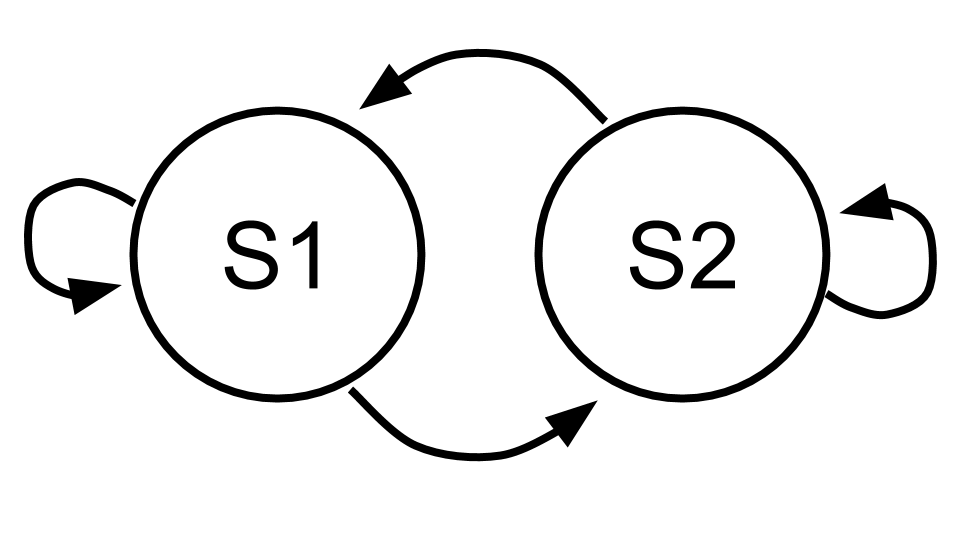
\includegraphics[scale=0.2]{./figs/chain_twostate.png}
\caption{}
\label{fig:two_state_mdp}
\end{figure}

Let's assume for now that we have a uniform posterior over these possibilities, thus $p= (1/3, 1/3, 1/3)$ and 
\begin{equation}
R = \begin{bmatrix}
0. &  0.5 & 0.5 \\
 1. & 0. & 0.5 \\
 0. & 0.5 & 0.  \\
 0. &  0. & 0. \\
\end{bmatrix}
\end{equation}

We will also assume for now that $u_E = \zero$. Thus we just want to find the robust solution that maximizes the $\avar$ of $\rho(\pi, R)$.

\subsection{Solutions for different $\alpha$}
Let's try solving for the optimal cvar policy for different values of $\alpha$. 

\begin{center}
\begin{tabular}{cccccc}
\hline 
$\alpha$ & CVaR & $P(\leftarrow \mid S1)$ & $P(\rightarrow \mid S1)$ & $P(\leftarrow \mid S2)$ & $P(\rightarrow \mid S2)$ \\ 
\hline 
0 & 0.75 & 1 & 0 & 1 & 0 \\
0.2& 0.70 & 0.6 & 0.4 & 1 & 0 \\
 0.5& 0.66 & 0.6 & 0.4 & 1 & 0 \\
 0.8& 0.66 & 0.75 &  0.25 & 1 & 0 \\
  0.99& 0.66 & 0.75 & 0.25 & 1 & 0 \\
\hline 
\end{tabular} 
\end{center}

As expected the CVaR decreases as $\alpha$ increases. However, I was surprised that it plateaued at 2/3 so quickly. 

\subsection{$q^*$ for different $\alpha$}
I also calculated $q^*$ for different $\alpha$ values.


\begin{center}
\begin{tabular}{c|c|cccc|ccc}
\hline 
$\alpha$ & CVaR & $r(S1, \leftarrow)$ & $r(S2,\leftarrow)$ & $r(S1, \rightarrow)$ & $r(S2, \rightarrow)$ & $q_1$ & $q_2$ & $q_3$\\ 
\hline 
0 & 0.75 & 1/3 & 1/2 & 1/6 & 0 & 1/3 & 1/3 & 1/3 \\
0.2& 0.70 & 0.35 & 0.44 & 0.21 & 0.0 & 0.29 & 0.42 & 0.29 \\
 0.5& 0.66 & 0.42 & 0.25 & 0.33 & 0.0 & 0.17 & 0.67 & 0.17 \\
 0.8& 0.66 & 0.25 & 0.5 & 0.25 & 0.0 & 0.5 & 0.5 & 0 \\
  0.99& 0.66 & 0.25 & 0.5 & 0.25 & 0.0 & 0.5 & 0.5 & 0 \\
\hline 
\end{tabular} 
\end{center}

\subsection{Numerical issues}
I've found that depending on the solver I use I sometimes get different answers. In particular, I ran with $\alpha - 0.2$ using either simplex or interior point and got two different results. The CVaR values are the same for both, and the CVaR maximizing policies are the same, but the values for $q^*$ are different. I think this is because the policy returns over the posterior are $\rho(\pi^*_{cvar},R) = [0.75 , 0.625, 0.75 ]$ for $R_1$, $R_2$, and $R_3$, respectively.

When choosing $q^*$ it will put as much mass on $R_2$ as possible, but then has a choice between $R_1$ and $R_3$ and it doesn't matter in terms of the robust representation. However, it does matter in terms of the actual reward function $R_{cvar} = \Ex_{R \sim q\opt}[R]$.

For simplex I get $R_{cvar} = (0.29, 0.5, 0.21, 0)$, but for interior point I get $R_{cvar} = (0.35, 0.44, 0.21, 0)$. Maximizing the first leads to always going right in S1 and left in S2. Optimizing the second leads to always going left in S1 and S2. Also the expected returns of each of the policies are different from the value of the CVaR objective and also different from the value of the robust representation LP objective with $\pi^*$ fixed. This seems problematic, if we can't recover the CVaR optimal policy from the CVaR reward since for $\alpha=0.2$ the solution of the CVaR LP was $\pi^* = (0.6, 0.4, 1, 0)$.
 
 
\section{Bayesian IRL}

We solve for the feature expectations using the following linear program~\cite{Puterman2005}:
	\[\max_{u:\states\times\actions\to\Real} \left\{ r\tr u ~\mid~ \sum_{a\in\mathcal{A}} (\eye - \gamma\cdot P_a\tr) u_a = p_0, u \ge \zero \right\}~. \]
	
For vanilla Bayesian IRL we need to get the Q-values for all states in the demonstrations. However, for optimizing CVaR and finding something robust to the best policy under each reward function we need the occupancy frequencies for each mdp in the chain. 

How do we do this? We take a hypothesis reward function $r$ and then run the above LP to get $u$. We then calculate the Q-values how? What's the fastest way with matrix vector notation? We can solve for values with LP, but then need to solve the dual for occupancy frequencies or can we recover them?

Can we efficiently go backwards? If we have the state value function, we can easily solve for the Q-values using an expectimax over next states. The Q-values give a greedy optimal policy. We can then solve for the feature expectations or state occupancies via a policy evaluation step. Actually, can't we just solve for the successor features via value iteration? This gives everything we need, right? Rather than using a scalar as the reward, just use a vector of state occupancies and dot with reward weights when computing max? This way seems better since we can get expected occupancies by taking initial distribution and multiplying by successor features matrix. 

\textbf{First TODO:}
Get slow version of BIRL working with running an LP for occupancy frequencies (dual). Then get policy, and policy rewards. Then we can solve for the value function as 
\begin{equation}
v_\pi = (I - \gamma P_\pi)^{-1} r_\pi
\end{equation}
and for the Q-values as
\begin{equation}
q_\pi(s,a) = r(s,a) + \gamma \sum_{s'} P(s,a,s') v_\pi(s')
\end{equation}
Alternatively, we can vectorize and solve as 
\begin{eqnarray}
q_\pi = r + \gamma 
\begin{bmatrix}
P_{a_1} \\
\vdots \\
P_{a_n}
\end{bmatrix}
 v_\pi
 = r + \gamma 
\begin{bmatrix}
P_{a_1} \\
\vdots \\
P_{a_n}
\end{bmatrix}
(I - \gamma P_\pi)^{-1} r_\pi
\end{eqnarray}


\textbf{Optimization TODO: }
Test this. Write a value iteration method that computes successor representations [Dayan, DeepMind] and check if I get the same thing as the LP.

Can probably use sparse matrices for transitions and make things faster!

Might want to transition to C++ if things are working nicely but too slow...

\section{Efficient Frontier}
Currently we just find a policy that has maximum CVaR. But what if we want to trade off how much risk or reward our policy has? Then we get a familiy of solutions. 

We need to change our objective so that we can balance expected return and risk. Then given different weights on the two objectives we get a curve of policies that maximize the expected return for a given risk tolerance or that minimize the risk given a certain lower bound on expected return. We can formalize this via a lagrange multiplier in the objective where we now want to maximize CVaR and maximize expected return over the distribution. \textbf{Question, do we want to do this over the mean or MAP reward?} Currently, I'm going to try over the mean reward of the posterior. Thus, the objective becomes:

	\begin{equation} \label{eq:lp_objective}
	\max_{u,\sigma} \left\{ \sigma -\frac{1}{1-\alpha} p\tr \left[\sigma\cdot\one - R\tr u  + R\tr u_E \right]_+ + \lambda \bar{r}^T u ~\mid~ \sum_{a\in\mathcal{A}} (\eye - \gamma\cdot P_a\tr) u_a = p_0, u \ge \zero \right\}~.  
	\end{equation}

Where $\bar{r} = Rp$, the mean reward under the posterior and $\lambda>0$ is a hyperparameter determining how much we value expected return over risk minimization. However, we can also use the MAP reward, if desired.

Okay, so how does this perform for different values of $\lambda$? I'm going to try this on the ambiguous lava domain from my AAAI'18 paper. 

\begin{eqnarray}
\min_{\sigma, u}&& -\sigma + \frac{1}{1-\alpha}p\tr z - \lambda p\tr R\tr u \\
\text{s.t.}&& - R\tr u + \sigma \one  - z  \leq -R\tr u_E\\
&&\begin{bmatrix}
(I - \gamma P_{a_1}\tr), \ldots, (I - \gamma P_{a_m}\tr)
\end{bmatrix}
\begin{bmatrix}
u_{a_1} \\
\vdots\\
u_{a_n}
\end{bmatrix}
= p_0 \\
&& u \geq \zero \\
&& z \geq \zero 
\end{eqnarray}	


\subsection{Experiment}
Let's try a range of lambdas for a fixed alpha and plot them. 
Let's also try a range of alphas with lambda = 0 and plot them. 
My hypothesis is that as lambda goes to infinity this will correspond to alpha = 0. Not sure what will happen in between, though.

To do this we take an MDP and calculate the optimal occupancy frequencies. We then need to save the CVaR and expected return of the policy and then plot them.

One interesting thing is that now the objective value is not the CVaR!!! It's got the expected return in it. So I need to just take the first part 
$CVaR = \sigma -\frac{1}{1-\alpha} p\tr \left[\sigma\cdot\one - R\tr u  + R\tr u_E \right]_+$



\section{Questions}
What to do about reward scaling? Can we add a L1 constraint to the LP? Taking a convex combo of $R_i$ could lead to a reward with $\|R\|<1$. I'm not sure if that is a problem or not.


What if we don't have good expert occupancies?
Can we do what we did in the AAAI'18 paper and have things relative to optimal policies for each posterior sample? Yes. this should work. What if the demonstrator is risky? Can we do better than the demonstrator but still stay safe? \textbf{I think this would be very compelling since other work like RS-GAIL just tries to match the safety of the demonstrator.}

Can we combine this with T-REX? We can get fast MCMC done with TREX maybe even add stein variational stuff. Then we have posterior. Can we make the demonstrations the baseline? Could take the empirical feature counts of the demos and try to maximize CVaR with respect to demonstrator.  

Since $\alpha=0$ is just maximizing CVaR over the entire distribution, isn't this just maximizing expected return? At least in the robust setting where $u_E = 0$? So if we have a lambda term on expected return versus isn't this effectively just scaling $\alpha$ \textbf{TODO: } Is there a difference empirically?

Okay, so here are the results for the ambiguous lava example. I ran Bayesian IRL with featurized linear reward to collect 2000 samples from the posterior. I then used a burn of 50 and skipped every other sample to form the final posterior. I solved for the CVaR optimal policy using several different values of $\alpha$ an using $\lambda \in [0.0, 0.01, 0.05, 0.075, 0.1, 0.2, 0.5, 0.75, 1.0, 2.0, 3.0, 5.0, 10.0, 100.0]$. The figures shown in Figure~\ref{fig:lava_ambiguous_frontiers} show the results along with the corresponding first lambda value that achieved a certain CVaR and expected return.

As expected we see a frontier of optimal policies that optimally trade-off robustness (lower CVaR is worse so higher CVaR is more robust) and expected return. Anything down and to the left of this efficient frontier curve will be dominated since it will either have the same robustness but lower expected return or the same expected return but lower robustness.

Surprisingly, there are not many optimal policies as you vary $\lambda$. But there are only two features, so I imagine that using more features will give more variety.

\begin{figure}
\centering
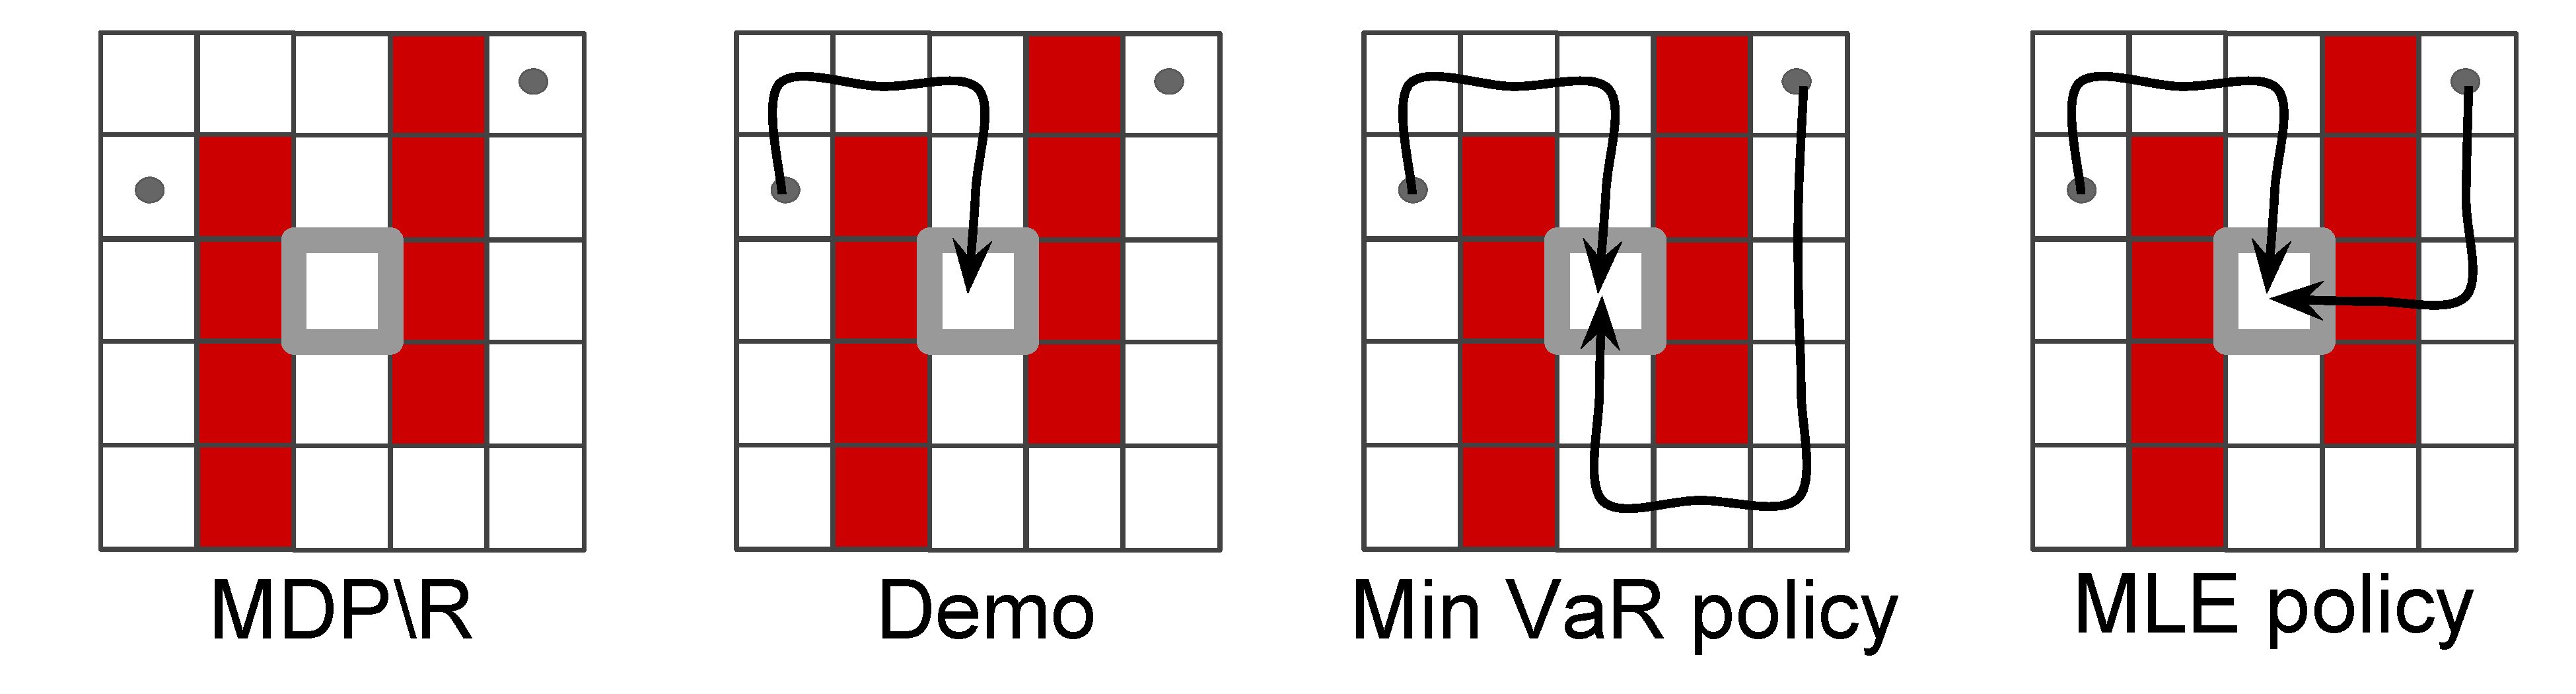
\includegraphics[width=0.75\linewidth]{figs/ImprovementWorld_revised.pdf}
\caption{}
\label{}
\end{figure}


\begin{figure}
     \centering
     \begin{subfigure}[b]{0.49\textwidth}
         \centering
         \includegraphics[width=\textwidth]{figs/{alpha0.75_lavaambiguous}.png}
         \caption{$\alpha = 0.75$}
         \label{fig:y equals x}
     \end{subfigure}
     \hfill
     \begin{subfigure}[b]{0.49\textwidth}
         \centering
         \includegraphics[width=\textwidth]{figs/{alpha0.9_lavaambiguous}.png}
         \caption{$\alpha = 0.9$}
         \label{fig:three sin x}
     \end{subfigure}
     \hfill
     
     \begin{subfigure}[b]{0.49\textwidth}
         \centering
         \includegraphics[width=\textwidth]{figs/{alpha0.95_lavaambiguous}.png}
         \caption{$\alpha = 0.95$}
         \label{fig:five over x}
     \end{subfigure}
          \begin{subfigure}[b]{0.49\textwidth}
         \centering
         \includegraphics[width=\textwidth]{figs/{alpha0.99_lavaambiguous}.png}
         \caption{$\alpha = 0.99$}
         \label{fig:five over x}
     \end{subfigure}
        \caption{Pareto Optimal Policies given different risk-tolerances.}
        \label{fig:lava_ambiguous_frontiers}
\end{figure}


One thing that I'm confused about is why we need $\alpha$ and $\lambda$. They seem similar, but I get different plots depending on the values. If alpha = 0, then the CVaR is the expected return. I'm going to try running multiple alphas with lambda fixed to zero to see what happens.
The restuls are in Figure~\ref{fig:varying_alpha}. It shows that higher alpha result in worse expected return and also worse CVaR. This makes sense since CVaR is adversarial wrt alpha.

\begin{figure}
\centering
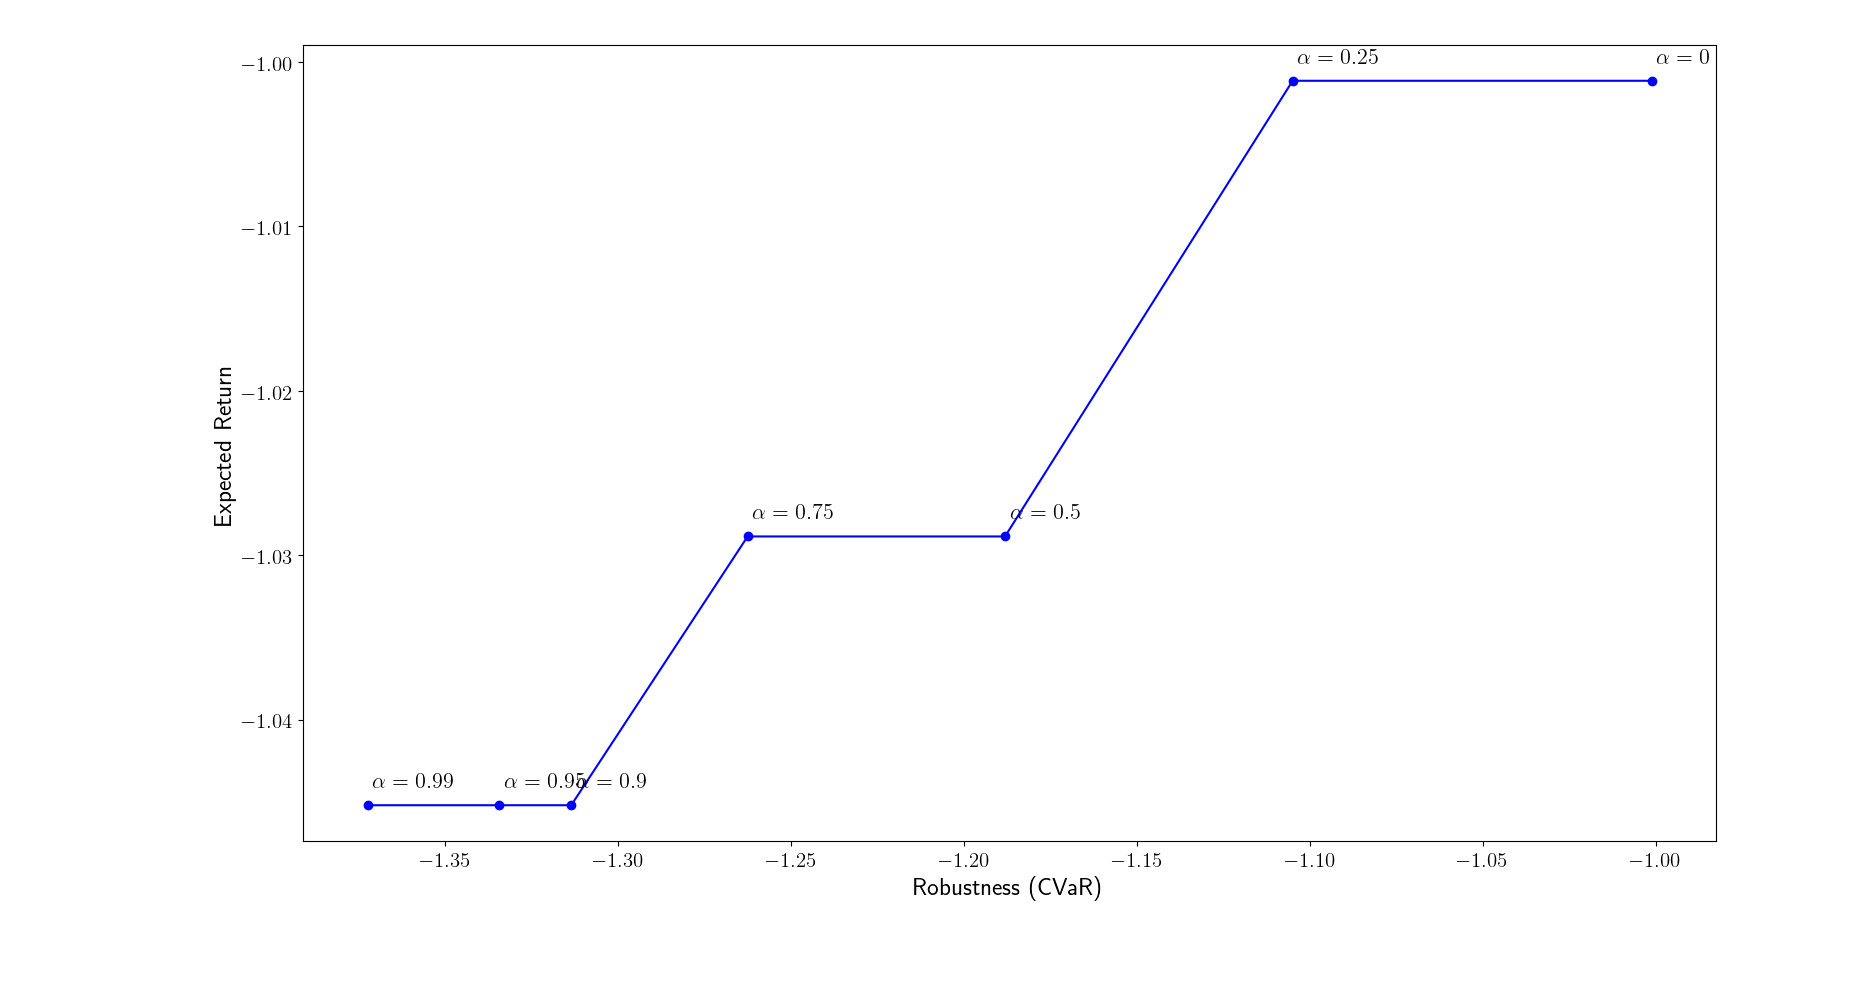
\includegraphics[width=\linewidth]{figs/alpha_range.png}
\caption{Varying $\alpha$ with $\lambda = 0$.}
\label{fig:varying_alpha}
\end{figure}




Another interesting thing is how the policy changes. I need to do some coding to get a better policy visualizer that allows for stochastic policies, but basically, what I see is that for small alpha it avoids red for but large alpha it takes the shortcut through red. It seems that the tail risk is over white features not red. The MAP reward gives a high penalty to white features to make the demonstration look more likely. This seems like a problem with Bayesian IRL. I wonder if using a MaxEnt flavor would help since then it wouldn't care as much about state-action pairs but about full trajectories? 



	
\section{TODO}
Extend this to linear feature approximation.

Extend to non-linear feature approximation via GAIL-like approach.



\bibliographystyle{plain}
\bibliography{library}
	
\end{document}